\section{Short-term Planning}

\hspace{2cm} The path that will be followed by the robot is a sequence of nodes, the current node can be decision or non-decision node. Our main controller will decide according to the robot state what is the appropriate action the robot should take by switching between three modules, classical control, learning control and obstacle avoidance at appropriate time to help the robot to reach the final destination. We will discuss each module separately in this section.

\subsection{Classical Control}

\hspace{2cm} The classical control theory uses a mathematical model to define the relationships between the input and output of a system. The most common type of these controllers are PID controllers. After they take the output of the system and compare it with the desired input, they generate an appropriate control signal based on the calculated error value.\cite{classical_control} A PID controller (proportional–integral–derivative controller) used to calculate the error which represent the difference between the setpoint (desired value ) and the measured variable and applies the correction.

In our project, we use classical methods to control the robot at intersection points on the map as shown in figure \ref{fig:intersetion points}. 
   \begin{figure}[H]%
    \center%
    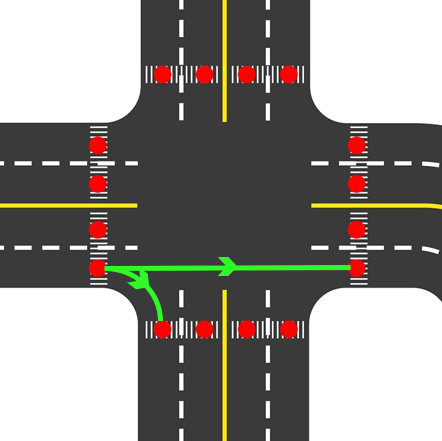
\includegraphics[width=.5\textwidth]
    {images/Alzahraa/intersectionPoints.png}%
    \caption[Map's Intersection Points]{Intersection points}\label{fig:intersetion points}%
  \end{figure}
  
With the help of state estimator that will be explained in section \ref{stateEstimator}, the current pose of the robot is determined and respectively the current node in path which tells if a decision has to be made at this node or not. If it is a decision node, the responsibility of controlling the robot is set to classical control.\\
The next node is retrieved from path and by calculating the distance between current and next node we can calculate the radius of curvature (R). \\
The linear velocity of the robot is constant and has the same value that is generated from the CNN model, so the required angular velocity to move the robot to the next node can be determined from this formula: $ w = v / R$.\\

\begin{figure}[H]%
    \center%
    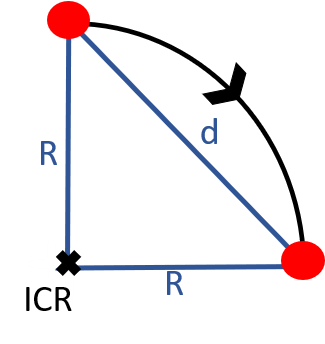
\includegraphics[width=.3\textwidth]
    {images/Alzahraa/classical.png}%
    \caption[Classical Control]{Determining value of angular velocity}\label{fig:w calculation}%
  \end{figure}

\subsection{Learning Control}
\hspace{2cm} imitation learning is considered one of the way of controlling autonomous cars that integrates prior driving experiences – a system that will help the cars perform on the road.
 car in the right

imitation learning can be used to train a convolutional neural network that maps perceptual inputs to
control commands; for example, mapping camera images to
velocity and the angle of velocity. This approach has been applied to lane following.
this will be discussed in section\ref{learn} .

\subsection{Obstacle Avoidance}
\hspace{2cm} In robotics, obstacle avoidance is the task of satisfying some control objective subject to non-intersection or non-collision position constraints. In unmanned air vehicles, it is a hot topic.What is critical about obstacle avoidance concept in this area is the growing need of usage of unmanned aerial vehicles in urban areas for especially military applications where it can be very useful in city wars. Normally obstacle avoidance is considered to be distinct from path planning in that one is usually implemented as a reactive control law while the other involves the pre-computation of an obstacle-free path which a controller will then guide a robot along. With recent advanced in the autonomous vehicles sector, a good and dependable obstacle avoidance feature of a driverless platform is also required to have a robust obstacle detection module.\cite{web038}

\par
In our project, we simply detect the obstacles by using LIDAR sensor only. LIDAR sensor gives the range between it and the obstacle and compare this range with a threshold to generate an appropriate linear and angular velocities that will help the robot to avoid this obstacle at appropriate time as shown in the figure below.
We used "testbot\_description" ROS Package to implement obstacle avoidance.
\par


 \begin{figure}[H]%
    \center%
    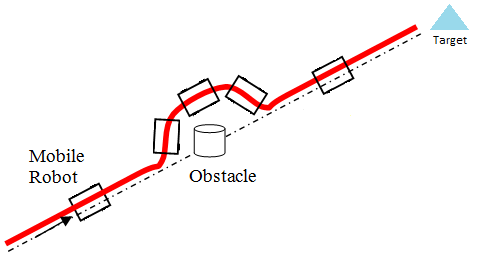
\includegraphics[width=.8\textwidth]{images/Alaa/Obstacle-avoidance.png}%
     % you need to add the caption for the list of figures
    \caption[obstacle avoidance]{The scenario of obstacle avoidance.}\label{fig: obstacle avoidance}%
  \end{figure}
 